\chapter{Introduction}~\label{ch01_introduction}

We are doing interesting things with biological filters.  I really don't know what to write in the introduction and that worries me.

Selective filters are everywhere in biology.  Examples of selective filters include the nuclear pore complex, diffusion in the nucleus, things moving through mucus barriers, drug delivery, liquid-liquid phase separation, and things like that.

Things I need to explain in the introduction: intrinsically disordered proteins, mostly.  Can that go in the nuclear pore intro?

\section{The nuclear pore complex is a unique selective filter}

The nuclear pore complex (NPC) is the filter that regulates all transport between the cell's nucleus and its cytoplasm.  Its unusual selective properties are apparent as it prevents significant flux of macromolecules larger than about 30 kDa ($\sim$ 5 nm) \cite{timney16}.  However, a class of proteins known as transport factors carry cargo molecules quite rapidy across the pore, although the complex of transport factor and cargo can be up to 40 nm in size.  Far from being a typical size-exclusion filter, therefore, the nuclear pore complex is a highly specific selective barrier which the cell uses to tightly control passage in and out of the nucleus. While the important biochemical components of nuclear transport have been identified, the mechanism of selectivity is still not well understood.  Even though the precise mechanism is under debate, it is clear that the NPC is a fascinating example of the cell leveraging intrinsically disordered proteins to accomplish a unique task.

\subsection{Intrinsically disordered proteins}

It has been long-standing conventional wisdom among biologists that a protein's folded shape determined its function.  Most enzymes and other proteins that were studied had a stable folded configuration, the lowest point on a well-defined folding energy landscape.  A protein's conformation provided specific docking points through which it could interact with ligands or other proteins in a ``lock-and-key'' model.

However, a few decades ago, it began to become clear that not all proteins have a well-defined ternary or even secondary structure, but rather exist as extended polymer chains.  These intrinsically disordered proteins (IDPs) were initially dismissed as nonfunctional, but evidence began to accumulate that they were in fact essential for cellular function, overturning the structure-function paradigm.  Their roles and importance are still being understood, as are the unusual mechanisms by which they accomplish their functions without a well-defined structure.

Today, it is estimated that 30\% of eukaryotic proteins are disordered or contain significant disordered regions \cite{uversky13}.  While there is significant sequence heterogeneity among IDPs, they tend to contain a large proportion of hydrophilic residues, and often have long stretches of low-complexity regions where only a few amino acids are represented.  They also often have high net charge.

Some IDPs fold (or partially fold) upon binding with an ordered partner, while others form ``fuzzy'' complex that remains disordered.  Their advantages over folded proteins may include their plasticity, which enables them to bind many different binding partners.  Multivalency, either as one-to-many or many-to-one binding, may also play a role.  They may act as hubs that bring together larger complexes.  Similarly, IDPs are often known for having high specificity at relatively weak binding strengths \cite{wright15, aramburu17}.

While the normal functioning of IDPs is very important to the cell, IDPs are also prone to aggregation and are at the root of pathologies such as Alzheimer's disease, Parkinsons, and prion diseases \cite{babu11}.  Often, normally-disordered proteins aggregate into amyloid fibrils, a stable structure based on parallel beta-sheets.

IDPs are commonly involved in cell signaling and regulation \cite{wright15}.  Their disordered nature makes them useful as hubs that bring together many other proteins, and as scaffolds that many proteins can bind to at once.  IDPs appear to be prevalent in transcriptional regulation, and they are playing increasingly apparent roles in liquid-liquid phase separation within cells \cite{brangwynne15}.  One of the most fascinating examples of IDP function is in the nuclear pore complex (NPC), a unique selective barrier that regulates all transport between the nucleus and the cytoplasm.  The link between disorder and selectivity is not well understood in this case.

\subsection{Basics of nuclear transport}

The nuclear pore complex (NPC) resides in the nuclear envelope of eukaryotes and regulates all macromolecular traffic between the nucleus and cytoplasm (Fig.~\ref{fig:NPC}).  The NPC is one of the largest protein complexes in the cell, at about 60 MDa in yeast and 120 MDa in humans \cite{beck17}.  As the regulator of nucleocytoplasmic transport, the NPC must rapidly and specifically allow a wide array of macromolecules to pass: transcription factors into the nucleus, and RNA into the cytoplasm.  It must also be robust to problems and able to accomodate mechanical strain as the nuclear envelope changes shape, as well as accomodating large cargo.  These functions are accomplished through a structure with two main parts, both made of proteins known as nucloporins, or Nups: the scaffold Nups, which form a ringlike complex, and the FG Nups, which are disordered and fill the central channel created by the scaffold Nups (Fig.~\ref{fig:NPC}).  

\begin{figure}
\centering
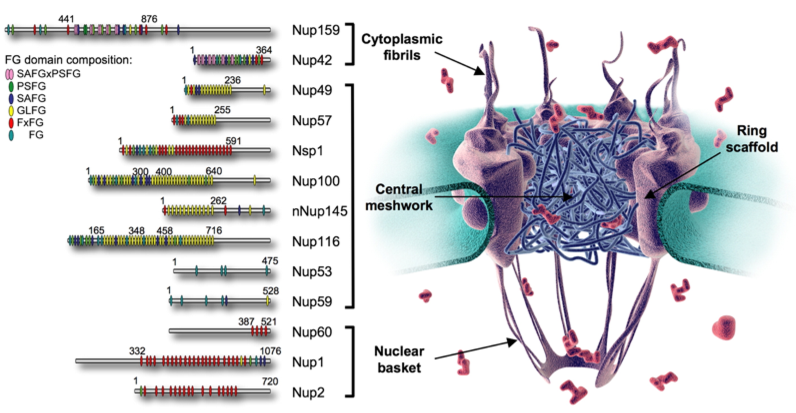
\includegraphics[width=\textwidth]{figs/ch01/patel.pdf}
\caption[Nuclear pore complex and FG Nups.]{Nuclear pore complex and FG Nups.  The cartoon shows the role of the FG Nups filling the central channel.  The left panel shows a schematic of the sequence of important FG Nups and the locations of their FG motifs. Figure adapted from \cite{patel07}.}
\label{fig:NPC}
\end{figure}

%There are about 30 different types of Nups, all present in multiple copy numbers.

The nuclear pore itself is formed of scaffold Nups, which are ordered proteins that form ringlike complexes with eightfold symmetry \cite{beck17,strambio-de-castillia10}.  The central channel of the pore is filled with disordered FG Nups.  FG Nups typically consist of an ordered domain that anchors them to the wall of the channel, and an entirely disordered domain that extends into the channel.  As with all Nups, FG Nups have eightfold symmetry in the pore, and some of them are present in much higher copy number. The disordered portion of every FG Nup contains phenylalanine- glycine (FG) motifs which bind to the hydrophobic binding pockets of transport factors.  While there are multiple binding motifs, all are short sequences which incorporate an FG repeat; for instance, FSFG, GLFG, and others.  Each FG Nup contains tens of FG repeats, leading to a high density of FG repeats within the pore \cite{strambio-de-castillia10,terry09}.

Since the FG Nups are disordered, most conventional visualization techniques, such as cryogenic electron microscopy and x-ray crystallography, are ineffective.  When imaged over time or when several pores are imaged, the averaged results do not show the disordered portion of the FG Nups. Techniques such as NMR and atomic force microscopy (AFM) can help gain insight into their conformational ensembles, as can some superresolution microscopy techniques, though the time and length scales of transport are often prohibitive for any microscopy \cite{hough15,sakiyama16,tu11}.  Early research suggested that the FG Nups formed a central plug or "transporter", but more recent work suggests that there is no central structure and the central channel is filled instead with highly dynamic disordered proteins \cite{moussavi-baygi16,schoch12,sakiyama16}. There is some evidence from simulations that the density of the FG Nups, as well as their charge density and hydrophobic properties, are not uniform along either the radial or axial directions \cite{yamada10,ando14,tagliazucchi13}.  This may contribute to selective transport, although the pore still functions without the asymmetric FG Nups \cite{zeitler04}.  Indeed, the NPC is remarkably robust to FG Nup deletion.  Over half of the mass of FG Nups can be removed without eliminating the selectivity barrier \cite{strawn04, zeitler04,kowalczyk11, jovanovic-talisman09}.

Transport factors (TFs) are ordered proteins that carry cargo through the NPC.  While there are various types, they share several features in common, most notably the fact that all known transport factors have more than one hydrophobic binding pocket which binds to FG repeats.  Binding affinities between TFs and FG Nups are surprisingly difficult to measure accurately.  Values of the dissociation constant $K_D$ measured outside of the cellular context are often in the low nanomolar range, implying a binding lifetime which is inconsistent with the experimentally-observed rapid translocation through the nuclear pore \cite{pyhtila03, gilchrist02}.  Recent consensus is that binding is much weaker in the cellular environment, with $K_D$ values between hundreds of micromolar and millimolar \cite{tetenbaum-novatt12-1, milles15, hayama18}.  The extreme binding multivalency of Nup - transport factor interactions adds a further layer of complexity to interpreting affinity data.  It is increasingly accepted that the highly transient and multivalent binding of TFs to FG Nups is key to the combination of high specificity and rapid transport exhibited by the NPC \cite{jovanovic-talisman17}.

The karyopherins (Kaps), also known as importins and exportins, are largest family of transport factors.  The approximately twenty different Kaps are responsible for most nucleocytoplasmic transport \cite{kapinos17}. Kaps typically consist of multiple HEAT repeats, a helical motif which conveys structural flexibility \cite{yoshimura16}.  Most Kaps bind their cargo directly via a nuclear localization signal (NLS, for nuclear import) or nuclear export signal (NES, for nuclear export).  NLS and NES are relatively short amino acid tags found on cargo \cite{chook11}.  However, sometimes the adaptor protein importin $\alpha$ is also needed.    In general, Kaps are on the order of 100 kDa in size, well above the passive permeability limit \cite{timney16}.   As discussed below, there is evidence that the presence of Kaps contributes to the selectivity barrier \cite{kapinos18,kapinos17,schleicher14, kapinos14}.  Many Kaps must be actively released from the nuclear pore and from their cargo after transit \cite{gorlich96,stewart07}.

%They are also known collectively as the importin $\beta$ superfamily \cite{tu11}.    

Unlike the karyopherins, nuclear transport factor 2 (NTF2) does not transport a wide variety of cargo across the NPC.  Instead, NFT2 maintains the Ran gradient needed for transport by carrying RanGDP across the pore \cite{ribbeck98,bayliss99}.  NTF2 is a homodimer whose monomers are 14 kDa and contain at least one FG binding site apiece.  Although its small size of 28 kDa is near the 30 kDa cutoff for passive transit through the pore, its flux through the pore is still at least 30 times that of similarly-sized proteins that do not bind to FG Nups \cite{ribbeck01,siebrasse02,kiskin03}.  NTF2 does not require adaptor proteins or active release from the pore. We predominantly use NTF2 as a model transport factor in both the theoretical and experimental work discussed here, because of its simplicity as well as its ease of expression and purification from bacterial cells.

Selective transport requires an energy source, which in the case of the NPC is provided by the Ran cycle.  When a TF-cargo complex passes from the cytoplasm into the nucleus, it encounters a RanGTP on the nuclear side which binds to the TF and displaces the cargo, actively releasing it.  Then the TF-RanGTP complex can collect a cargo destined for nuclear export, and this ternary complex can diffuse back through the NPC to the cytoplasm.  The protein RanGAP then hydrolyzes the RanGTP to RanGDP, disrupting the complex into its three original pieces.  Ultimately, the energy source for selective nuclear transport comes from the RanGTP-RanGDP gradient from the cytoplasm to the nucleus, a gradient which is maintained partially by NTF2, which carries RanGDP through the pore \cite{jovanovic-talisman17,stanley17}.  From the perspective of transport, this means that the process of passing through the pore is itself passive and does not consume energy.  The selectivity ultimately arises from concentration gradients maintained by the Ran cycle, but the selective mechanism is not itself active.

One surprising feature of nuclear transport is its sheer speed and volume.  The high macromolecular traffic between nucleus and cytoplasm requires high flux through each NPC.  Experiments with permeabilized cells estimate that the total molecular flow through the NPC could be as high as 10-20 MDa per pore per second, corresponding to roughly 1000 transport events per pore per second \cite{ribbeck01}.  Experiments focusing particularly on NTF2 report fluxes between 50 and 250 molecules per pore per second \cite{ribbeck01, siebrasse02, kiskin03}.  Fluxes this high mean a continuously high occupancy of the NPC, estimated at around 100 karyopherins at once \cite{paradise07}. One reason that individual NPCs can accomodate such high flux is the rapidity with which molecules transit the pore.  A wide range of molecules, such as NTF2, Importin $\beta$, and GFP-NLS cargoes, have a dwell time of less than 10 ms in the pore \cite{tu11, yang06, dange08, kubitscheck05}.  Typically, this is determined using single-molecule tracking with superresolution microscopy \cite{tu11}.

%The flux through an NPC is determined not only by the transit time, but also by the success rate of transit attempts.  Single-molecule microscopy suggests that the nuclear import efficiency of Importin $\beta$ ranges from 50\% to 80\%, depending on concentration \cite{yang06}.  Modeling supports these numbers \cite{zilman07}.

%%%%%%
 % I feel like I've been seeing more new simulations than new experiments recently.  The sliding NTF2 paper was pretty good, and Zilman's stuff is interesting.  I thought the passive-diffusion-limit paper by Timney was good too.  The Milles paper from 2015 which focuses on the ultrafast binding kinetics is quite helpful.  I've been seeing several structure papers for the NPC as a whole, which aren't super interesting to me.  The thermo paper from the Rout lab was fascinating because they used ITC on exactly the same NTF2 and FSFG constructs that we did.  I should compare their results to ours more closely, because I'm not sure why they could get publishable data and we couldn't.  Probably I was just bad at ITC, but it merits closer investigation.  One paper I really hated was that AFM paper from a few years ago.  Sure, it's cool that they can even approach the temporal and spatial resolution needed to image the pore, but they were nowhere near fast enough to say anything meaningful about transport or Nup conformations.  Also they didn't run any negative controls.

%And I just remembered the Gorlich one about phase separation in that one Nup.  I forget if they were liquid droplets at any point, but at some point they were clearly aggregates because they weren't spherical at all.

%There is an inner ring and two outer rings, the nuclear and cytoplasmic rings.  The outer rings are slightly larger.  The nuclear ring is on the side of the nucleus and includes the nuclear basket.  The cytoplasmic ring includes the cytoplasmic filaments, which are (probably?) disordered proteins extending out into the cytoplasm.
%
%The eightfold symmetry of the pore arises from its modular nature.  Scaffold Nups form various stable subcomplexes, of which one of the most important is the Y-complex.  The Y-complex forms the inner ring; there are 32 copies of the complex per pore \cite{beck17}.  The rings themselves are relatively flexible, as they need to be in order to accomodate deformations of the nuclear envelope.  This flexibility is achieved in part by through short linear motifs (SLMs) which connect the subcomplexes to each other.
%
%Recent cryo-EM studies have achieved unprecedented resolution of the scaffold Nups \cite{rout study, other EM study}.
%
%% Scaffold Nups have very low turnover rates. \cite{knockenhauer16}
%% 2000-3000 copies of NPC in an average human cell. \cite{knockenhauer16}
%%''The mass flow through NPCs in proliferating HeLa cells is estimated to be 10–20 MDa·NPC−1·s−1 `` verbatim from \cite{tu11}
%% Largest cargos are 40 nm also has a citation in Tu SM review article 2011
%
%\subsection{FG nucleoporins are disordered and fill the central channel of the pore.}

\subsection{Models of nuclear transport}

While the components of nuclear transport are well-understood, the mechanism behind its unusual selective properties is unclear.  Broadly speaking, two of the most important theoretical frameworks are the hydrogel model and the entropic barrier model (Fig.~\ref{fig:hydrogel-entropic-brush}).  Both are supported by some experimental results and challenged by others, and they are not mutually exclusive.  Both could contribute to selective transport.

\begin{SCfigure}
\centering
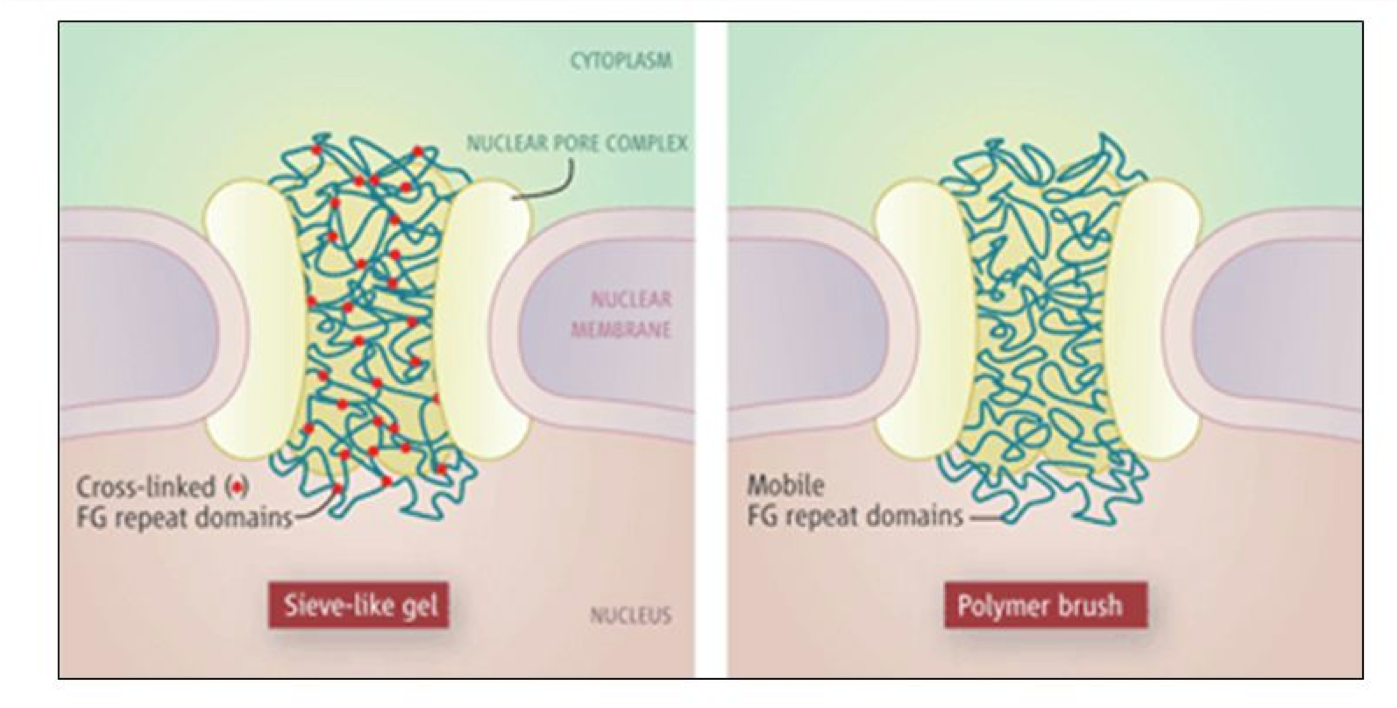
\includegraphics[width=0.6\linewidth]{figs/ch01/elbaum}
\caption[Two important models of nuclear transport.]{The two major models of the nuclear pore: the hydrogel (sieve-like gel) and entroptic barrier (polymer brush) models. Figure from \cite{elbaum06}.}
\label{fig:hydrogel-entropic-brush}
\end{SCfigure}

The hydrogel model posits that the FG Nups within the nuclear pore are transiently crosslinked at their FG repeats into a hydrogel-like structure.  Inert proteins are prevented from passing through the pore due to the small mesh size, while transport factors carrying cargo can also bind to the FG repeats, disrupting the hydrogel and moving through the pore.  This view of the nuclear pore is supported by experiments showing that the disordered domain of the essential FG Nup Nsp1 aggregates into a hydrogel when purified into buffer \cite{frey06}.  These hydrogels show strong selectivity for import of transport factors and their cargo over inert proteins, demonstrating binding between the aggregated FG Nups and the transport factors \cite{frey07,ader10,kim15}.  Theoretical models of diffusion through a transiently-crosslinked hydrogel show selective properties \cite{ribbeck01, bickel02,gu19}.   However, while nuclear pore mimics which consist of aggregrated FG Nups display highly selective entry of transport factors, they do not permit the exit of transport factors over timescales consistent with transport \cite{frey07,ader10}.  Furthermore, some Nups which aggregate in buffer remain disordered in the cellular environment \cite{hough15}.

Conversely, the entropic barrier model supposes that FG Nups instead act as polymer brushes within the pore.  In this view, inert proteins are prevented from entering the pore due to the entropic penalty they would incur by restricting the possible conformations of the Nups.  However, the decrease in free energy upon a transport factor binding to a Nup offsets the entropic penalty and allows transports and their cargo to pass \cite{rout00, lim08}.  Evidence for this view comes from a number of studies in which single layers of FG Nups are grafted onto a surface and their extension monitored as transport factors are titrated on and off the surface \cite{wagner15,zahn16,vovk16}.  Layer height tends to change non-monotonically as transport factors are added, suggesting that the presence of transport factors affects the selectivity of the nuclear pore.

% wagner 15 is the paper with the weird binding maps

More generally, FG Nups exist on a continuum of ``cohesiveness,'' ranging from Nups (or portions of Nups) which do not aggregate at all under pretty much any conditions to ones which do so readily \cite{hough15}.  Nup cohesiveness depends on their charge, length, and hydrophobicity.  Many simulations of the nuclear pore aim to understand the role of Nup cohesiveness in transport \cite{gu19,tagliazucchi13,nasrabad16,mincer11}.  There may be distinct regions of differing Nup properties within the nuclear pore.  A relatively common method of modeling transport is to computationally reduce the problem to that of a transport factor diffusing in a one-dimensional effective potential representing its interactions with Nups (Fig~\ref{fig:effective-potential}) \cite{tagliazucchi13, zilman07,tu13, timney16}.  These models predict selective transport while being highly dependent on the precise details of Nup composition and location within the nuclear pore.  These models also do not presuppose that either the hydrogel or entropic brush model is fully correct, but allow for a mixture of cohesive and non-cohesive Nups.

\begin{SCfigure}
\centering
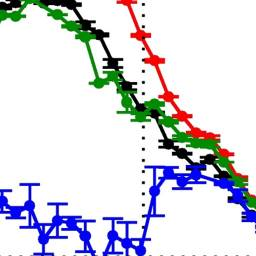
\includegraphics[width=0.5\linewidth]{figs/ch01/tagliazucchi}
\caption[Effective potential model of nuclear transport.]{Example of effective-potential model of nuclear transport.  Figure shows simulated free-energy landscape for a variety of possible transport factors as a function of position within the nuclear pore. Figure from \cite{tagliazucchi13}.\\}
\label{fig:effective-potential}
\end{SCfigure}

Apart from the question of FG Nup conformation within the nuclear pore, the role of transport factors themselves in the permeability barrier has been under investigation \cite{kapinos18,kapinos17,schleicher14,kapinos14}.  There is evidence that the presence of karyopherins (Kaps) in the nuclear pore increases its selectivity for transport factors, possibily by establishing ``tight-binding'' and ``weak-binding'' subpopulations of Kaps which compete for binding sites on the Nups \cite{wagner15}.  Even non-specific ompetition may make the nuclear pore's selectivity barrier more robust as well \cite{tetenbaum-novatt12,zilman09,zilman10,timney06}.  The precise role of crowding and competition in nuclear pore selectivity is fascinating but as yet unclear.

%\begin{SCfigure}
%\centering
%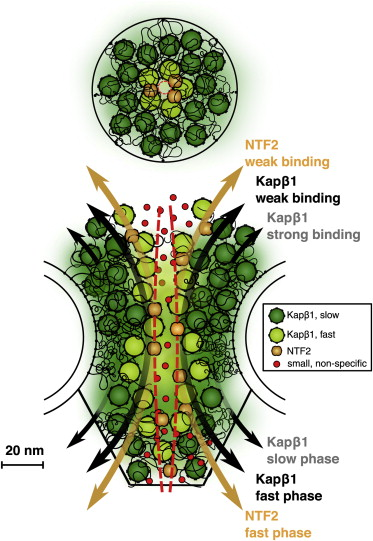
\includegraphics[width=0.4\linewidth]{figs/ch01/Kap-centric-lim}
%\caption[Two important models of nuclear transport.]{The two major models of the nuclear pore \cite{elbaum06}}
%\label{fig:hydrogel-entropic-brush}
%\end{SCfigure}

Relatively few non-computational, quantitative theories of nuclear transport exist.  Reaction-diffusion models have been proposed with varying degrees of complexity and different underlying assumptions but they do not take both binding kinetics and binding site saturation into account \cite{yang18,zilman07}.

%I don't think there's too much in the way of MD simulations, it's mostly coarse-grained stuff because of the scale of the pore.  The Raveh sliding paper is an exception, and they weren't really looking at transport.

%There are a few intermediate models of the pore that combine features of the hydrogel and brush, like the reduction of dimensionality and forest models.

% md simulations \cite{pulupa17,vovk16}

\subsection{Artificial nuclear pore mimics}

Systems which mimic the selectivity of the nuclear pore have been attempted using a wide range of approaches, with mixed success.  Some nuclear pore mimics recreate the nanopore geometry of the NPC \cite{jovanovic-talisman09,ananth18a}.  Several others are based on hydrogels, whether hydrogels composed of aggregated FG Nups \cite{frey07,ader10, kim15} or inert hydrogels with tethered Nups or Nup-derived peptides \cite{yang18,friedman16a}.  There was an interesting study using DNA origami to mimic the scaffold of the nuclear pore, with multiple FG Nup attachment sites, but that one is just a proof of concept right now \cite{fisher18}.  While these mimics have all shown selectivity to some extent, none have definitively shown a flux of transport factors through the pore that matches that observed experimentally.  
%One of Loren's colleagues in New York grafted FG Nups onto a gold-coated nanopore and monitored flux through the pore.  She saw low (less than 10-fold) selectivity.  I'm not sure whether other nanopore-based approaches have been tried.

\section{Other selective biofilters}
\label{sec:other-systems}

Selective biofilters exist in many contexts outside of nuclear transport, and they frequently include a common set of elements that are exemplified by the nuclear pore.  In particular, cells often need proteins to move rapidly within a cellular compartment but still possess high binding specificity.  This is often accomplished with intrinsically disordered proteins that interact transiently and multivalently with their binding partners.  In the crowded environment of the cell or extracellular matrix, nonspecific binding can immobilize proteins, hindering selective motion, unless those proteins are able to continue diffusing while bound, a feature which we argue is key to the selective transport of the NPC as well as the biofilters discussed here. The following section presents three particular examples of selectivity in biological systems, from widely disparate areas, which bear striking similarities to the selectivity of the nuclear pore.  In the remainder of this work, we model selective transport using a minimal set of characteristics that, while inspired by the nuclear pore, apply to all of the systems here as well.

\subsection{Drug delivery through mucus barriers}

One medically-important selective biological barrier is the mucus which lines organs such as the lungs, nose, and stomach.  In particular, lung mucus presents a barrier to delivery of inhaled medication.  If nanoparticles containing drugs for lung diseases such as asthma and lung cancer could be inhaled and taken up by lung cells, doses could be lower, as the uptake would be more targeted \cite{carlson18,schneider17}.  However, lungs are coated by a layer of mucus intended to prevent foreign objects from reaching the lung cells.  In order to deliver nanoparticles to lung cells, they must be engineered to pass the selective mucus barrier.

Mucus consists predominantly of disordered glyocoproteins known as mucins, though other components such as lipids are present as well \cite{witten17}.  These entangled mucins present multiple barriers to nanoparticles, as shown in Fig.~\ref{fig:mucus}.  First, large particles are excluded due to the 150-350 nm average pore size of mucus gels \cite{lai10,lai11}.  Second, even particles which are small enough to enter the mucus layer often bind to mucins.  In fact, mucoadhesive particles (MAPs) have been specifically engineered on the principle that increasing the nanoparticle's lifetime within the mucus will lead to more efficient drug delivery \cite{peppas85}.  However, diffusion of MAPs is often so slow that they do not penetrate beyond the edge of the mucus layer.  Furthermore, mucus gradually replaces itself on clearing timescales which vary depending on the type of mucus.  Nanoparticles in the outermost region will be cleared more rapidly than those which diffuse deeply into the mucus layer \cite{lay03}.

\begin{figure}
\centering
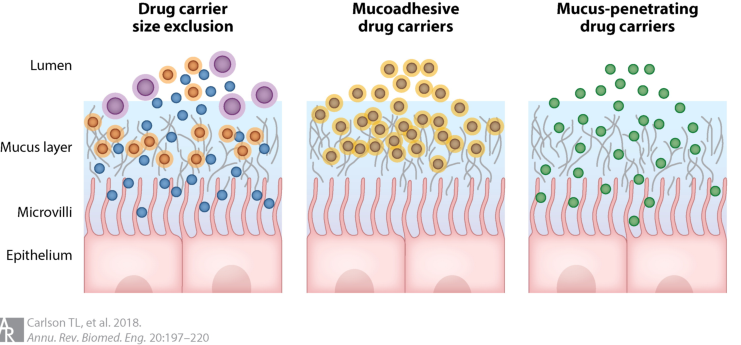
\includegraphics[width=0.8\linewidth]{figs/ch01/carlson-mucus.pdf}
\caption[Nanoparticle drug delivery through a mucus barrier.]{ Nanoparticle drug delivery through a mucus barrier.  Particles which are too large cannot pass the size-exclusion barrier.  Mucoadhesive particles penetrate the mucus layer but are trapped by binding interactions.  Inert mucus-penetrating particles have a much higher diffusion constant in mucus.  Figure adapted from \cite{carlson18,popov16}}
\label{fig:mucus}
\end{figure}

Currently, the best nanoparticle delivery through the lung mucus barrier is by small, inert particles which minimize nonspecific interactions with mucins.  These mucus-penetration particles (MPPs) are typically coated in PEG or another inert polymer \cite{schneider17, huang17}.  MPPs can reach much higher diffusion constants in mucus than can MAPs \cite{mastorakos15,lai11,porsio18,tang09}.

The selective barrier of lung mucus bears similarities to the selectivity of the nuclear pore in that it consists of disordered proteins which bind to particles impinging on the barrier.  However, in the case of mucus, binding inhibits the flux of particles through the selective filter, while binding enhances the flux of transport factors through the nuclear pore.  A better understanding of the role of binding and bound diffusion to a selective filter such as the nuclear pore could suggest novel strategies for nanoparticle delivery through lung mucus.  Perhaps binding can be leveraged in a way that enhances nanoparticle flux over that of inert particles, improving drug delivery to the lungs.

\subsection{Diffusion of DNA-binding proteins in the nucleus}

The principles of selective filtering in the nuclear pore appear in biological systems beyond straightforward filtering.  In particular, transient binding and bound-state diffusion are important to DNA targeting in the nucleus by transcription factors and DNA damage repair proteins.  A protein diffusing in the cell's nucleus has many of the same constraints and capabilities as a transport factor transiting the nuclear pore: it is surrounded by a high concentration of flexible tethers to which it binds transiently.  Just as this situation leads, counterintuitively, to high flux of transport factors through the nuclear pore, DNA-targeting proteins find their specific targets much more rapidly than would be naively predicted \cite{mirny09}.  

Solutions to this ``needle in the haystack'' challenge resemble possible mechanisms of bound diffusion in the nuclear pore complex.  In particular, it is widely accepted that the search for targets is made more rapid through facilitated diffusion, involving proteins sliding along strands of DNA.  However, the optimal time spent in a one-dimensional search as opposed to a free three-dimensional search is unclear; as is the effectiveness of sliding as opposed to multiple, rapid binding and unbinding events \cite{halford09}.  This mechanism is reminiscent of both the sliding mechanism predicted in some transport factors and of the effect of diffusion while bound to a flexible tether \cite{raveh16}.  Additionally, transfer of a multivalent transcription factor between two strands of chromatin, a mechanism known as intersegmental hopping, can increase the protein's search space similarly to the multivalent inter-Nup hopping that is available to transport factors \cite{doucleff08,halford04a}.  Finally, transient binding plays an important role in the search for DNA targets.  This speed-stability paradox reflects the fact that, like in the nuclear pore, proteins must bind very weakly to their DNA tethers to avoid becoming immobile.  Unlike nuclear transport, however, DNA-binding proteins must bind more tightly to their targets upon reaching them \cite{iwahara13,zandarashvili15}.

A case in point, further discussed in Sec.~\ref{sec:parp1}, is that of poly(ADP-ribose) polymerase 1 (PARP1), a DNA damage repair protein which rapidly localizes to sites of DNA damage.  PARP1 binds damaged DNA with low nanomolar affinities, and appears to bind undamaged DNA only a few orders of magnitude more weakly \cite{sukhanova16}.  Given that there are up to 5 mM nonspecific DNA binding sites in the nucleus, the speed with which PARP1 diffuses ($\sim$ 10 times slower than in buffer) is remarkable \cite{iwahara13}.  PARP1 contains multiple DNA-binding sites, and an inter-strand hopping mechanism has recently been demonstrated, which may explain its rapid diffusion \cite{rudolph18}.  However, removal of that mechanism only slightly slows the recruitment of PARP1 to sites of DNA damage, suggesting that a further mechanism of bound-state diffusion is necessary \cite{mahadevan18}.  The principles of selective nuclear transport may help to explain the rapid motion of PARP1, along with other DNA damage repair proteins and transcription factors.

%Also, some people have done modeling on the optimal compaction and number of loops for this kind of diffusion search \cite{cortini18}. 

\subsection{Subcompartments in liquid-liquid phase separated droplets}

\begin{figure}
\centering
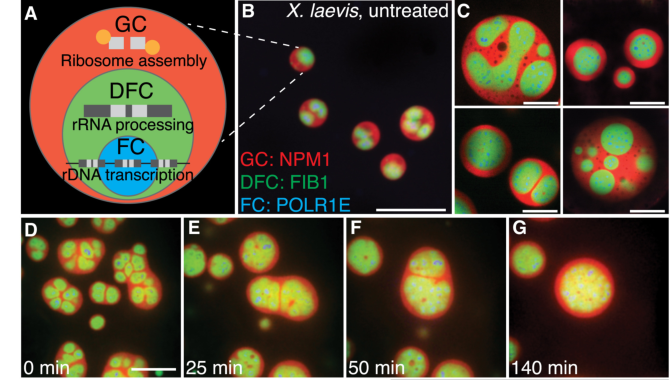
\includegraphics[width=0.8\linewidth]{figs/ch01/feric16.pdf}
\caption[Phase-separated subcompartments of the nucleolus.]{ Phase-separated subcompartments of \textit{Xenopus} nucleolus. (A) Schematic of subcompartments. (B)-(C) Fluorescence microscopy image of nucleoli with subcompartments in red, green, and blue. (D)-(G) Time-course showing dissolution of compartments after actin disruption. Figure adapted from \cite{feric16}.}
\label{fig:nucleolus}
\end{figure}

Features of nuclear transport such as highly-concentrated disordered proteins and bound-state diffusion also appear in liquid-liquid phase separated droplets.  These membraneless organelles are rapidly gaining prominance as it becomes clear that many cellular functions are regulated through the phase separation of mixtures into phase rich in various proteins and other cellular components.  Membraneless organelles include nucleoli, which aid in processing ribosomal DNA genes within the nucleus, and RNA granules, which help sort mRNA \cite{shiina19, brangwynne15}.

Liquid-liquid phase separation typically occurs for mixtures containing IDPs with ``sticker'' and ``spacer'' regions, similar to the hydrophobic FG repeats and hydrophilic linker regions in FG Nups \cite{posey18}.  These phases are highly concentrated, but the proteins that comprise them remain mobile.  Interestingly, evidence is developing for subcompartments of varying composition within some liquid droplets.  Nucleoli contain multiple subcompartments which are thought to perform distinct functions (Fig.~\ref{fig:nucleolus}) \cite{feric16,catalano15,oday19}, while RNA granules have recently also been shown to have a core-shell structure \cite{jain16,shiina19}.

The investigation of subcompartments in membraneless organelles is in its very early stages, with much of the current work going towards simply identifying the components of the compartments.  Discussion of their purpose and mechanisms is still quite speculative.  However, it seems plausible that one function of these compartments is to selectively concentrate enzymes or other proteins to increase reaction rates.  RNA bodies in particular are known to sort and sequester mRNA \cite{shiina19}.  As such, the presence of disordered, multivalent proteins may not simply be necessary for the formation of phase separated droplets, but could potentially assist in selectively filtering the components of the subcompartments.  If nuclear transport is a guide, binding partners of the IDPs which form the outermost phase might have a higher flux into the inner compartments than nonbinding proteins.  Additionally, in the context of bound-state diffusion, liquid droplets represent maximal bound diffusion, as binding to an IDP in solution will not appreciably slow the diffusion of the binding partner.  While these possibilities will not be testable for some time, membraneless organelles may prove to be a fascinating application of selective biofiltering.

\section{Project goals and motivation}

All of the systems described above involve the rapid flux of proteins which still bind highly selectively to their environment.  This apparent paradox further includes common features such as ultrafast, transient, multivalent binding and the presence of binding sites on flexible, dynamic tethers.  The mechanism by which these features lead to such remarkable selective properties is not obvious.  We approached the problem through both modeling and experiment and identified a common key parameter in the form of bound-state diffusion.  While the theory and experimental setup were based on nuclear transport, both platforms are general enough to apply to a number of selective biofilters.

\subsection{Model selective transport as simply as possible}

Despite the complexity of nuclear transport, many components can be removed or approximated without eliminating its unusual selective properties.   For example, Nups which are asymmetrically distributed along the axis of the nuclear pore can be removed, as can a large fraction of Nups overall, without destroying selectivity \cite{strawn04, zeitler04,kowalczyk11, jovanovic-talisman09}.  And though many transport factors require active release from the pore, others, such as NTF2, do not; selectivity is not therefore dependent on active release.  We decided to model the pore in order to answer the question: What are the minimum requirements for selective transport?

In the course of creating the model, we found that the minimum requirements are quite simple indeed.  The model discussed in Chapter~\ref{ch02} not only dispenses with non-uniformly distributed Nups and facilitated release, but also with non-specific crowding, Kap-centric control of the nuclear pore, the Ran cycle, and even the nanopore geometry.  Instead, the pore is treated as a bulk material of finite thickness with an artificially-imposed concentration gradient to drive flux across it.  Competition for binding sites is retained in the form of binding site saturation, but even without this feature we see selective flux across the barrier.  Our model fundamentally contains only diffusion and binding of transport factors to Nups - an extremely streamlined depiction of nuclear transport, and one that can even be treated semi-analytically.

The simplicity of our model made the key parameter clear: we could not reproduce the selectivity of the nuclear pore without allowing bound-state diffusion, that is, assuming that bound Nup - transport factor complexes were mobile within the pore.  Bound diffusion provides a possible answer to the paradox of nuclear transport, resulting in a higher flux of transport factors, which bind to Nups, than inert proteins which do not.  In our model, this straightforward mechanism alone gave rise to the decidedly unintuitive behavior of the nuclear pore.

Having identified bound-state diffusion as an important parameter for selective filters, we investigated possible methods of bound diffusion within the nuclear pore.  Two possibilities arose from basic, well-accepted facts of nuclear transport: tethered diffusion arising from the disordered, flexible nature of the Nups, and inter-chain hopping of the transport factor due to its binding multivalency.  Upon investigation, both mechanisms can plausibly provide the high bound diffusion constant needed to reproduce the selectivity of the nuclear pore.

While this model was inspired by nuclear transport, it ultimately relies on only a few key properties of the system.  With this model, we predict selective transport will occur where there is bound-state diffusion, which can be readily obtained if flexible IDPs are present for tethered diffusion, or if highly transient, multivalent binding allows for moving from one site to another while remaining bound.  The systems described above in Sec.~\ref{sec:other-systems} fall into this category, as likely do many others.  Furthermore, these principles might guide synthetic selective biofilters with novel rapid, highly-selective properties.

\subsection{Experimentally test bound-state diffusion in biomaterials}

After developing the minimal model of selectivity, we began developing a synthetic biofilter with which to experimentally probe the effect of bound-state diffusion  on selectivity.  The model itself is sufficiently general to apply to a wide range of filters, giving us some freedom in designing a material to test its predictions.  We chose to use the nuclear pore as inspiration for this material because its key components are so well known, if not well understood.  In order to capture the key features of selectivity, we designed hydrogels containing peptide tethers derived from FG Nups.  The transport factor NTF2 served as a test protein whose diffusion we could compare with a similarly-size but nonbinding counterpart.  These hydrogel nuclear pore mimics display the mechanisms that lead to selective transport in our model: flexible, dynamic tethers which can transiently bind to transport factors, along with multivalent transport factors which can ``hop'' between peptide chains without fully unbinding.  We predict that these features will be sufficient for bound-state diffusion of the transport factor within the hydrogel.

As with the theoretical model, many of the NPC-specific details, such as the nanopore structure and Ran gradient, were omitted.  A bulk material was used instead of nanopores because our model should apply equally well to both, and a macroscopic hydrogel is much easier to study.  We quickly realized that hydrogels are a challenging system to use for protein separation.  The nuclear pore mimics have a rigorous set of competing constraints: for example, the hydrogel should be in mechanical equlibrium and homogeneous, while still well-sealed to a flow chamber so that proteins cannot bypass the gel.  Chapter~\ref{ch03} documents the design of the hydrogel nuclear pore mimics.  Many modifications intended to improve the diffusion properties and reproducibility of the hydrogels proved unsuitable for our needs.  However, we eventually produced a biomaterial that can be used to measure bound diffusion, while also developing more general guidelines for designing hydrogels that are useful for protein separation.

The resulting bound-state diffusion measurements are presented in Chapter~\ref{ch:bound-diffusion}.  Fluorescence recovery after photobleaching (FRAP) was used to determine the effective diffusion constants of both NTF2 and an inert protein, from which the bound diffusion constant was calculated.  The data analysis ultimately required a two-dimensional Fourier series solution to the diffusion equation, resulting in a set of data-processing scripts which can be applied to any circular material undergoing equilibration with a fluorophore.  We measured a non-zero bound diffusion constant that is consistent with the predictions of our model, and tested the effect of varying Nup length on bound-state diffusion.  Our results indicate that these nuclear-pore-inspired hydrogels can be used to probe the effect of our model's parameters on bound diffusion.

While bound diffusion is a key parameter in our selectivity model, the aggregation state of the Nups could also affect selectivity.  Aggregated Nups will be less dynamic and effectively act as shorter tethers, limiting bound diffusion.  In Chapter~\ref{ch05}, we probed the aggregation behavior of an FG-Nup-derived peptide in several crowded conditions.  Using a fluorescent amyloid assay, we identified significant differences in the aggregation dynamics in the presence of different crowders, including between poly(ethylene glycol) (PEG) and polyvinylpyrrolidone (PVP), two inert polymers that are widely presumed to be interchangeable as crowders.  We followed this aggregation assay with NMR and fluorimetry studies in order to investigate the nature of the changes.  The results suggest that the presence of an aromatic ring in PVP may interact with the phenylalanines in the FG motifs of the peptide, changing its local chemical environment and therefore its aggregation behavior.

Although a true hydrogel-based selective biofilter proved challenging to design, our nuclear-pore-inspired material can be used to measure the bound-state diffusion of proteins.  This parameter is likely important to a variety of problems involving rapid transit of highly-selective proteins.  It is my hope that the model and biomaterials developed here can be used to investigate these systems more generally in the future.  This work suggests that bound-state diffusion, particularly when resulting from transient, multivalent binding, may explain a number of fascinating biological paradoxes.

\section{Biophysics is beautiful}

Nuclear transport, besides being a well-studied example of all of the above properties as they relate to selective transport, is an extremely fascinating process, full of counterintuitive results and apparent paradoxes.  The nuclear pore is at once an incredibly intricate nano-machine and also astoundingly robust to perturbation.  Passage through the nuclear pore is carefully controlled by complex cellular processes and requires constant energy input, yet the mechanism of selectivity itself is both passive and highly unusual.  Even NTF2, right at the edge of the passive permeability limit, gets through about 30 times faster than GFP.  With its relevant length scale on the order of a hundred nanometers and timescale of milliseconds, it's very difficult to visualize or probe.  Traditional biochemistry techniques don't work on it because the disordered proteins all average to zero.  And apparently quite unusually hydrophobic for disordered proteins.  The binding of Nups and transport factors is also extreme: extremely fast on-rate (as fast as you can get!), extremely weak (my understanding is that once you get into $K_D$'s of millimolar or hundreds of micromolars, most biochemists call that ``nonspecific binding'', so basically not binding at all), and extremely multivalent.  Binding between transport factors and Nups is decidedly \textit{not} a canonical, textbook protein-protein binding interaction.   It's a weird, nonintuitive system that produces weird, nonintuitive results.  I've never been able to explain nuclear transport to someone without them thinking it's really cool, and me agreeing.

%That sets up another cool point about this model of selectivity in general - pretty much every other filter I can think of works solely by blocking the things that shouldn't pass.  However, the nuclear pore, in our model, works by sterically blocking both transport factors and inert proteins.  They both get excluded by the Nups, by which I mean have their flux significantly reduced from what it would be through an empty channel of the same size.  But then the flux of transport factors separately gets boosted by an entirely different mechanism, often hundreds of times over the flux of the inert protein.  That would be sort of like, I'm having trouble coming up with a good macroscopic analogy, hmm, I don't know.  But it's a really weird and interesting property for a filter to have!  Usually the very best thing a filter can do is to act invisible to the thing that's passing through.  But here the filter actually enhances the flux.  I am trying hard to avoid using the phrase ``actively enhances the flux'' because that's not, strictly speaking, true.  We got rid of the explicit energy consumption along with all the other things we threw out.  So it's not really active transport, but it's exceedingly unusual passive transport.

There is also value in studying the nuclear pore specifically from the perspective of a physicist.  There is a constant tension in biophysics between the full, complex, messiness of any living system, and the drive to simplify and reduce it to it's smallest set of component parts.  As a physicist, I tend to come down more on the side of simplification.  Beyond all practical value, there's something extremely satisfying about applying simple theories to complex systems and getting meaningful results.  That can be anything from Cohen's flies and that one angular parameter that explains almost everything about how they right themselves after being knocked over.  Or the analysis of whale kinetic energy, or the scaling of the barbs in cat tongues, to how cucumber tendrils coil and overwind.  Not that the simple theory will get everything right, of course, but if you can predict even 60\% of a complicated thing by tuning one key parameter, that's beautiful.  We need the full complexity for life to work, but we also need the big, sweeping, simple, underlying principles.  And I think that applying them even to complicated things, which they manifestly can't explain thoroughly, is a really good way to leverage the simple underlying theories into practical advances.

So no matter how you look at it, there is much to be gained from a study of binding and diffusion in selective biofilters.  It's a unique process and could lead to novel technologies as well as new understanding.

%\section{Why everyone else is wrong}

%Starting with the papers most nearly related to our work, the Olsen group paper uses a really really similar model but does some weird things with the assumptions.  They only use the linear approximation, which might be good in the pore but Mike shows that it gets non-physical at surprisingly large values of $K_D$.  Just as troublingly, they allow flux of the bound complex out of the pore.  This would mean that Nups are constantly coming loose and drifting away into the cytoplasm all the time.  It makes the math simpler and gives a more elegant answer, but it really makes no sense at all physically.  Anton's paper doesn't make a mistake like that, but it does sweeping the binding kinetics under the rug.  It assumes that the on and off rate are infinitely fast compared to diffusion and therefore of necessity cannot probe the interesting things that happen when that's not true.  Furthermore, they actually do make an error by assuming chemical equilibrium in the presence of an artificial concentration gradient.  It makes all of their little Nup potentials into one big effective potential, but that's not allowed, mathematically.

%Zooming out a bit, most of the effective potential models are not super convincing to me.  Here I'm talking mostly about the coarse-grained simulation ones.  There are a ton of them (so I should find a lot and cite them) and I don't think they really agree with each other.  Furthermore, the answers depend a lot on the details they decide to include in the simulation.  Even if I trust them for the nuclear pore, they're not easily applied to any other system.  They require knowledge of the composition and location of Nups along the axis of the pore, and about the properties of the transport factors, and generally they are super-specialized.

%Looking at experiment, I don't have terribly many particular complaints, but it does bother me how the answers don't agree.  Of course we don't believe the hydrogel model as Gorlich presents it.  That's because of Loren's in-cell NMR experiments that show no aggregation of FG124, and also because it doesn't make too much sense.  I think Loren wrote up that bit in the theory paper supplement to show that it doesn't really make sense.  The affinities of the purified hydrogels for Nups are also way too strong.  Affinities in the nanomolar region would mean that the transport factors never get out of the hydrogel.  There's a nice figure in Loren's paper that shows the affinities that we would expect for things that get through on realistic timescales.  Add in the fact that nobody can even agree on the binding affinity for Nups and transport factors and I don't think that people really know what's going on.

%Apart from Gorlich's hydrogels, there are a number of SPR-type grafting experiments, although I haven't seen new ones like that in a while.  These give pretty much every result under the sun?  They stick Nups down to a surface and flow various transport factors across them.  The Nups extend, or sometimes contract, or sometimes contract and then extend, and everyone writes up discussion sections that make it sound like it's totally what they expected.  Somebody, I think Zilman, wrote up a theory paper that fits all the disparate results into it, which somehow just makes me a bit suspicious.  One thing that I am not actually suspicious about is that transport factors really do make a difference to NPC permeability.  I'm not sure I totally buy into the Kap-centric control thing, or that crowding is a key feature for selectivity, but there really does seem to be something there.  If I were to keep studying the nuclear pore in particular, I would next want to expand our selectivity model to try and take crowding and competition into account.

%Okay, what else has been showing up recently in the nuclear pore field?  People finally seem to be agreeing that the affinity has to be micromolar or millimolar, and I agree with that.  They've identified weak, transient, multivalent binding as a special form of selectivity.  I agree with that too.  I feel like I've been seeing more new simulations than new experiments recently.  The sliding NTF2 paper was pretty good, and Zilman's stuff is interesting.  I thought the passive-diffusion-limit paper by Timney was good too.  The Milles paper from 2015 which focuses on the ultrafast binding kinetics is quite helpful.  I've been seeing several structure papers for the NPC as a whole, which aren't super interesting to me.  The thermo paper from the Rout lab was fascinating because they used ITC on exactly the same NTF2 and FSFG constructs that we did.  I should compare their results to ours more closely, because I'm not sure why they could get publishable data and we couldn't.  Probably I was just bad at ITC, but it merits closer investigation.  One paper I really hated was that AFM paper from a few years ago.  Sure, it's cool that they can even approach the temporal and spatial resolution needed to image the pore, but they were nowhere near fast enough to say anything meaningful about transport or Nup conformations.  Also they didn't run any negative controls.

%And I just remembered the Gorlich one about phase separation in that one Nup.  I forget if they were liquid droplets at any point, but at some point they were clearly aggregates because they weren't spherical at all.

%There have been a handful of hydrogel NPC mimics as well, apart from the Gorlich ones.  The Kim/Ribbeck paper used that pentameric domain to make gels with tethered Nups.  There was another one that anchored just the FG motifs into the gels - I don't think that should work too well but I forget what they saw.  And the Olsen group paper where they did basically what we did but apparently without any of the troubleshooting.  I don't trust that one at all and I'm still upset.

%Overall, the biggest issue with the field as I see it is that everyone thinks they know what's going on.  There's been a shift recently towards both the hydrogel and the entropic brush camp both just kind of assuming they are right and it's been settled?  We kept getting reviewers who say that everyone knows this stuff, when I don't think that's actually true.  I'm pretty sure nobody really knows much, probably including us, but at least we are trying to remove all the distractions and focus on the simplest possible model.

%\section{Theoretical models of the nuclear pore}

%The big two are the hydrogel and the entropic brush model.  The hydrogel model is very strongly promulgated by Gorlich and I'm sure some other people but I'm not sure quite who.  Katharina Ribbeck too. This relies mostly on the fact that Nsp1 and some other Nups form hdyrogels in buffer that show strong selective enty for transport factors and their cargo \cite{frey06, frey07}.  The idea of cohesive Nups shows up in a lot of simulation papers too.  This is the idea that Nups form transient crosslinks between their FG repeats.  The transport factor also binds to those repeats, so it basically melts its way through the gel.  The Bruinsma paper and some of Zilman's work deal with diffusion through transient meshworks in a more theoretical way.  This is where Franck's work overlaps with ours.  I don't think he has anything published yet.  His work and Bruinsma both try to quantify diffusion in a transient meshwork with binding.  The hydrogel model hasn't actually shown diffusion of transport factors out of their artificial gels.

%The entropic brush model says that the Nups are not, in fact, crosslinked, but are extended polymers in the pore.  The inert proteins are then excluded by the entropic penalty that the Nups would incur if the proteins got into the pore and restricted the possible conformations they could take.  The free energy change of the transport factor upon binding to the Nups offsets this penalty.  The experimental evidence for this model is largely based on SPR studies where a single layer of Nups are grafted onto a surface, and then the layer height is monitored as binding partners are titrated in and out.  There's that paper with the weird binding maps, that should go in this part.  And Zilman's theoretical model of it, plus the papers with the actual binding studies.  Loren's NMR paper goes here too, because it shows that FG124 stays disordered in bacterial cells.

%The role of transport factors and crowding is a separate consideration from the hydrogel vs brush thing.  There's pretty good evidence at this point that the presence of transport factors makes the selective barrier more robust.  I'm unclear on the precise lines of reasoning, but one idea (probably in that binding map paper) says that there's a tightly-bound Kap population that basically just hangs out in the pore taking up binding sites, so that the mobile Kap population can't bind too strongly.  There's that pretty graphic from the Rout lab with all the Kaps in the pore.  The words ``Kap-centric control'' apply here.  Zilman has been doing a fair amount of work on crowding and competition lately and I should check up on that.  My takeaway right now is that the presence of Kaps definitely matters but I'm not sure how.

%The simulations and effective potential models are agnostic, mostly, towards the hydrogel vs. brush debate.  They just try to model the pore computationally and see what comes out.  I confess that I don't pay too much attention to most of these models.  The effective potential ones reduce the problem to a transport factor traveling through a 1-D potential.  There are several different papers but the underlying difference between them are unclear to me.  I don't think there's too much in the way of MD simulations, it's mostly coarse-grained stuff because of the scale of the pore.  The Raveh sliding paper is an exception, and they weren't really looking at transport.  I like that paper because it has pretty pictures and told us a thing we already thought was true.

%There are a few intermediate models of the pore that combine features of the hydrogel and brush, like the reduction of dimensionality and forest models.  I don't know too much about those.  Anton's phase-diagram kind of paper fits into this intermediate place too sort of.  I think that both features are probably important and I don't know of anyone who has explicitly tried to combine them in an analytic theory as opposed to simulation.

%\section{Why our model is cool}

%Mostly it's cool because it's so simple.  Nobody else in the field likes that idea.  But we got rid of almost everything and still made a selective material.  We got rid of the geometry, of the different types of Nups, of cargo and importin alpha and whatever, of Ran and active release.  We got rid of crowding and Kap-centered whatever, though we still did allow competition in the form of binding site saturation.  The linear model got rid of that too.  We really stripped the system down to basically nothing and still predicted that binding helps you pass through the pore more rapidly.  That's not at all intuitive.  It's worth talking about a bit more as a paradox.  It's very difficult to imagine a situation in which sticking to the environment that you're moving in helps you move faster.  Of course, it doesn't actually help you move faster.  It just increases the overall flux through the material at steady-state.  As we've seen with the model and the hydrogel mimics, the binding proteins actually move more slowly, as would be expected.  The binding really helps to get more of the transport factor into the pore and increases the total transport factor concentration right at the far edge.  That way, when transport factors unbind at the edge, they have a good chance at leaving the pore entirely.  And the bound mobility means that  - hmm, more stuff moves through.  It's hard to articulate in a strictly accurate way?  It's like having two populations of transport factor that equilibrate separately and both contribute to the flux, whereas the inert protein only has the unbound population.

%That sets up another cool point about this model of selectivity in general - pretty much every other filter I can think of works solely by blocking the things that shouldn't pass.  However, the nuclear pore, in our model, works by sterically blocking both transport factors and inert proteins.  They both get excluded by the Nups, by which I mean have their flux significantly reduced from what it would be through an empty channel of the same size.  But then the flux of transport factors separately gets boosted by an entirely different mechanism, often hundreds of times over the flux of the inert protein.  That would be sort of like, I'm having trouble coming up with a good macroscopic analogy, hmm, I don't know.  But it's a really weird and interesting property for a filter to have!  Usually the very best thing a filter can do is to act invisible to the thing that's passing through.  But here the filter actually enhances the flux.  I am trying hard to avoid using the phrase ``actively enhances the flux'' because that's not, strictly speaking, true.  We got rid of the explicit energy consumption along with all the other things we threw out.  So it's not really active transport, but it's exceedingly unusual passive transport.

%Another thing that has surprised me has been the ways this model applies to other systems, and not even just filtering systems.  I would not have thought of DNA binding proteins as terribly similar to our model, though I remember Loren getting me to look up some Xist stuff a long time ago, so maybe I'm the only one surprised.  But the PARP1 paradox is very similar to the NPC problem, and Johannes and the Lugar lab even came to the same conclusions we did, more or less.  And this new thing about vancomycin and the endlessly-shedding cell membrane for the MRSA bacteria.  There's no bound diffusion involved, but our model still helps predict why it should have antibiotic resistence.  That's plus the other drug-delivery applications and so on that I'll talk about elsewhere.  This is only the stuff that has basically fallen into our laps in the year or so since we developed the model.  I really do think it could be broadly applicable to a number of disparate biological problems.  Although the nuclear pore aspect of the project is going to end when I leave, I do hope that the lab can keep using this model and collaborating with other groups to investigate bound-state diffusion.  I don't believe in too much of what I've done here, but I believe that bound-state diffusion, particularly when resulting from transient, multivalent binding, can explain a number of biological paradoxes.

%\section{Next section}

%What else should go in the introduction?  It's getting harder to avoid talking about mucus and drug delivery, which I'm not really looking forward to because I don't know much about it.  Kathryn made a good point though, which is that I should pick two or three examples similar to the nuclear pore and write about them. PARP1 is going to be one, I guess.  And drug delivery through mucus, for which I'll find some interesting papers cited by \cite{witten17}.  Is there another one to write about?  If it were obvious, Loren and Meredith would have found it for the intro to the theory paper.  

%If I were really going to use the introduction to answer the question ``why did I do this work?'' the answer would probably just be the section above.  It's cool.  Nuclear transport really is a super interesting problem.  I keep getting discouraged by the whole thing, and then I try to explain it to someone and get interested all over again.  The nuclear pore is at once this incredibly intricate nanoscale machine and also extremely robust to perturbation.  It is really picky about what gets through, but it uses binding to encourage things to pass through.  Even NTF2, right at the edge of the passive permeability limit, gets through about 30 times faster than GFP.  Nobody can ``look'' at it with traditional biochemistry techniques because the Nups are disordered and average to zero.  The Nups are, as far as we know, really disordered even by the standards of disorder.  And apparently quite unusually hydrophobic for disordered proteins.  The binding of Nups and transport factors is also extreme: extremely fast on-rate (as fast as you can get!), extremely weak (my understanding is that once you get into $K_D$'s of millimolar or hundreds of micromolars, most biochemists call that ``nonspecific binding'', so basically not binding at all), and extremely multivalent.  We had absolutely no idea how to fit the ITC data, it was so multivalent.  I really should check on how the Rout group did it.  This is decidely NOT a well-studied, canonical, protein-protein binding interaction.  It's a weird, nonintuitive system that produces weird, nonintuitive results.  Who wouldn't want to understand it?

%And for me personally, the ``physics'' part of ``biophysics'' is also very important.  It's not where everyone is coming from, I know, but I got interested in biophysics because of complex systems that could be well-explained with simple theories.  Not that the simple theory will get everything right, of course, but if you can predict even 60\% of a complicated thing by tuning one key parameter, that's beautiful.  It's like Itai Cohen's flies and that one angular parameter that explains almost everything about how they right themselves after being knocked over.  Or the analysis of whale kinetic energy, or the scaling of the barbs in cat tongues.  Any time you can get a whole series of curves to collapse onto one, that's the beauty of biophysics.  I think that a lot of the biologists don't agree.  They think the complexity is the beauty, and I can't really argue, because we need the full complexity for life to work, but we also need the big, sweeping, simple, underlying principles.  And I think that applying them even to complicated things, which they manifestly can't explain thoroughly, is a really good way to leverage the simple underlying theories into practical advances.  Traditional physicists, on the other hand, sometimes disappoint me because they don't want to bother applying simple first principles to things that they manifestly cannot explain fully.  They want to focus on ``simple'' things like handfuls of really cold atoms (not that those are honestly simple) and just understand those really, really well.  That's super useful too, of course, and I'm glad somebody wants to do it.  That's how we get lasers, etc.  But somehow it seems like the biophysics that I like the most gets labeled as frivolous by both the physicists and the biologists.  I don't think it's frivolous.  I think it's astounding.

%Maybe my ultimate point here is that, despite being disillusioned with everything scientific right now, I get genuinely excited when explaining my work to people.  That has to mean something.


%
%
%
%
%%%%%%%%%%%%%%%%% IDPS %%%%%%%%%%%%%%%%%%
%
%\section{Intrinsically disordered proteins are essential to cellular function}
%For decades, it was conventional wisdom among biologists that a protein's folded shape determined its function.  Most enzymes and other proteins that were studied had a stable folded configuration, the lowest point on a well-defined folding energy landscape.  A protein's conformation provided specific docking points through which it could interact with ligands or other proteins in a ``lock-and-key'' model.
%
%However, a few decades ago, it began to become clear that not all proteins have a well-defined ternary or even secondary structure, but rather exist as extended polymer chains.  These intrinsically disordered proteins (IDPs) were initially dismissed as nonfunctional, but evidence began to accumulate that they were in fact essential for cellular function, overturning the structure-function paradigm \cite{uversky13}.  Their roles and importance are still being understood, as are the unusual mechanisms by which they accomplish their functions without a well-defined structure.
%
%Today, it is estimated that 30\% of eukaryotic proteins are disordered or contain significant disordered regions \cite{uversky13}.  While there is significant sequence heterogeneity among IDPs, they tend to contain a large proportion of hydrophilic residues, and often have long stretches of low-complexity regions where only a few amino acids are represented.  They also often have high net charge.
%
%Some IDPs fold (or partially fold) upon binding with an ordered partner, while others form ``fuzzy'' complex that remains disordered.  Their advantages over folded proteins may include their plasticity, which enables them to bind many different binding partners.  Multivalency, either as one-to-many or many-to-one binding, may also play a role.  They may act as hubs that bring together larger complexes.  Similarly, IDPs are often known for having high specificity at relatively weak binding strengths \cite{uversky13}.
%
%While the normal functioning of IDPs is very important to the cell, IDPs are also prone to aggregation and are at the root of pathologies such as Alzheimer's disease, Parkinsons, and prion diseases.  Often, normally-disordered proteins aggregate into amyloid fibrils, a stable structure based on parallel beta-sheets.
%
%IDPs are commonly involved in cell signaling and regulation \cite{uversky13}.  Their disordered nature makes them useful as hubs that bring together many other proteins, and as scaffolds that many proteins can bind to at once.  IDPs appear to be prevalent in transcriptional regulation, and they are playing increasingly apparent roles in liquid-liquid phase separation within cells.  One of the most fascinating examples of IDP function is in the nuclear pore complex (NPC), a unique selective barrier that regulates all transport between the nucleus and the cytoplasm.  The link between disorder and selectivity is not well understood in this case.
%
%%%%%%%%%%%%%%%%%%%% NUCLEAR PORE STRUCTURE %%%%%%%%%%
%
%\section{Major components of nucleocytoplasmic transport}
%The nuclear pore complex (NPC) resides in the nuclear envelope of eukaryotes and regulates all macromolecular traffic between the nucleus and cytoplasm.  The NPC is one of the largest protein complexes in the cell, at about 60 MDa in yeast and 120 MDa in humans \cite{beck17}.  As the regulator of nucleocytoplasmic transport, the NPC must rapidly and specifically pass a wide array of macromolecules: transcription factors into the nucleus, and RNA into the cytoplasm.  Moreover, it must be robust to problems and able to accomodate mechanical strain as the nuclear envelope changes shape, and to passage large cargo.
%
%A typical yeast cell has xx nuclear pores, each with a dimension of xx.  Human cells have about xx pores with xx dimensions.
%
%There are about 30 different types of Nups, all present in multiple copy numbers.
%
%These functions are accomplished through a structure with two main parts, both made of proteins known as nucloporins, or Nups: the scaffold Nups, which form a ringlike complex, and the FG Nups, which are disordered and fill the central channel created by the scaffold Nups.  Aside from the NPC itself, transport factors (TFs) are a class of proteins essential for selective transport.  The energetic cost of selectivity is captured in the Ran GTP/GDP cycle.
%
%\subsection{Scaffold nucleoporins are ordered and form ringlike complexes.}
%The nuclear pore itself is formed of scaffold Nups, which are ordered proteins that form ringlike complexes with eightfold symmetry \cite{beck17}.  There is an inner ring and two outer rings, the nuclear and cytoplasmic rings.  The outer rings are slightly larger.  The nuclear ring is on the side of the nucleus and includes the nuclear basket.  The cytoplasmic ring includes the cytoplasmic filaments, which are (probably?) disordered proteins extending out into the cytoplasm.
%
%The eightfold symmetry of the pore arises from its modular nature.  Scaffold Nups form various stable subcomplexes, of which one of the most important is the Y-complex.  The Y-complex forms the inner ring; there are 32 copies of the complex per pore \cite{beck17}.  The rings themselves are relatively flexible, as they need to be in order to accomodate deformations of the nuclear envelope.  This flexibility is achieved in part by through short linear motifs (SLMs) which connect the subcomplexes to each other.
%
%Recent cryo-EM studies have achieved unprecedented resolution of the scaffold Nups \cite{rout study, other EM study}.
%
%% Scaffold Nups have very low turnover rates. \cite{knockenhauer16}
%% 2000-3000 copies of NPC in an average human cell. \cite{knockenhauer16}
%%''The mass flow through NPCs in proliferating HeLa cells is estimated to be 10–20 MDa·NPC−1·s−1 `` verbatim from \cite{tu11}
%% Largest cargos are 40 nm also has a citation in Tu SM review article 2011
%
%\subsection{FG nucleoporins are disordered and fill the central channel of the pore.}
%The central channel of the pore is filled with disordered FG nucleoporins (FG Nups).  FG Nups typically consist of an ordered domain that anchors them to the wall of the channel, and an entirely disordered domain that extends into the channel.  As with all Nups, FG Nups have eightfold symmetry in the pore, and some of them are present in much higher copy number.
%
%The disordered portion of every FG Nup contains phenylalanine- glycine (FG) motifs which 
%bind to the hydrophobic binding pockets of transport factors.  While there are multiple binding motifs, all are short sequences which incorporate an FG repeat; for instance, FSFG, GLFG, and others. \cite{the rout paper I took that figure from}.  Each FG Nup contains x-x FG repeats, leading to an extremely high density of FG repeats within the pore.
%
%Since the FG Nups are disordered, most conventional visualization techniques do not work.  When imaged over time or when several pores are imaged, the averaged results do not show the disordered portion of the FG Nups.  Cryo-EM and x-ray crystallography don't work.  Techniques such as NMR and very fast AFM can help gain insight into their conformationa ensembles \cite{Loren's papers, the AFM paper}.  Early research suggested that the FG Nups formed a central plug or "transporter", but more recent work suggests that there is no central structure, just disordered proteins (the AFM study from Lim or Lemke group). There is some evidence from simulations that the density of the FG Nups, as well as their charge density and hydrophobic properties, are not uniform along either the radial or axial directions \cite{some energy landscape things, some simulations}.  This may contribute to selective transport, although the pore still functioned with all of the asymmetric FG Nups removed.  Indeed, the NPC is remarkably robust to FG Nup deletion.  Over half of the mass of FG Nups can be removed without eliminating the selectivity barrier \cite{beck17}.
%
%\subsection{Energy for selective transport is provided by the Ran cycle.}
%Selective transport requires an energy source, which in the case of the NPC is provided by the Ran cycle.  When a TF-cargo complex passes from the cytoplasm into the nucleus (nuclear import), it encounters a RanGTP on the nuclear side which binds to the TF and displaces the cargo.  Then the TF-RanGTP complex can collect a cargo destined for nuclear export, and this ternary complex can diffuse back through the NPC to the cytoplasm.  The protein RanGAP then hydrolyzes the RanGTP to RanGDP, disrupting the complex into its three original pieces.  Ultimately, the energy source for selective nuclear transport comes from the RanGTP-RanGDP gradient from the cytoplasm to the nucleus, a gradient which is maintained partially by NTF2, which carries RanGDP through the pore \cite{stanley17}.
%
%From the perspective of transport, this means that the process of passing through the pore is itself passive and does not consume energy.  The selectivity arises from concentration gradients maintained by the Ran cycle.
%
%\subsection{Transport factors}
%
%Transport factors (TFs) are ordered proteins that carry cargo through the NPC.  While there are various types, they share several features in common, most notably the fact that all known transport factors have more than one hydrophobic binding pocket which binds to FG repeats.  In fact, many TFs have several binding pockets.  Likewise, the binding affinity between TFs and FG Nups remains unknown for most TFs.  Estimates of dissociation constant $K_D$ vary from nanomolar to millimolar, depending on the environment (cellular, buffer, etc.) in which the measurement is made \cite{things}. There are many types of TF, of which some of the most important are the importins and exportins (karyopherins), NTF2, (and mRNA exporters? CRM? mex67?).
%
%The karyopherins (Kaps) are the most-studied family of TFs.  They are also known (in human cells?) as importins and exportins, or collectively as the importin $\beta$ superfamily \cite{tu11}.  The twenty or so different Kaps are responsible for most nucleocytoplasmic transport \cite{kapinos17}.  Kaps typically consist of multiple HEAT repeats, a helical motif which conveys structural flexibility \cite{yoshimura16}.  Most Kaps bind their cargo directly via a nuclear localization signal (NLS, for nuclear import) or nuclear export signal (NES, for nuclear export).  NLS and NES are 5-7 amino acid tags found on cargo \cite{}.  However, Kap95? (importin $\beta$) uses the adaptor protein Kap60? (importin $\alpha$) to bind its cargo. In general, Kaps are on the order of 100 kDa in size, well above the passive permeability limit \cite{}. Kaps may contribute to the selectivity barrier.
%
%Unlike the karyopherins, nuclear transport factor 2 (NTF2) does not transport a wide variety of cargo across the NPC.  Instead, NFT2 is focused on maintaining the Ran gradient needed for transport.  It transports RanGDP across the pore - why does this help maintain a gradient?  If it transports in both directions, wouldn't it help wash out the gradient?  NTF2 is a homodimer whose components are 14 kDa and have one FG binding site.  Although its small size of 28 kDa is near the 30 kDa cutoff for passive transit through the pore, its flux through the pore is still 30-150 that of similarly-sized proteins that do not bind to FG Nups.
%
%There are other TFs such as Mex67 and CRM, but I don't really know what they do.  Is RNA exported using Kaps or are there other TFs for that?
%
%%%%%%%%% EXPERIMENTAL OBSERVATIONS %%%%%%%%%%%%%%%
%%\section{Observed features of nucleocytoplasmic transport}
%%\subsection{Flux through the NPC is very high.}
%%\subsection{TFs show millisecond dwell times.}
%%\subsection{TF-FG Nup binding kinetics are ultrafast.}
%%\subsection{FG Nups may take a variety of conformations.}
%%    \subsubsection{Grafted layer heights change when TFs are added.}
%%    \subsubsection{Inter-Nup cohesion varies between FG Nups.}
%%\subsection{TF concentration and crowding may affect selectivity.}
%%\subsection{The NPC is also a passive permeability barrier.}
%%\subsection{A detailed, mechanistic picture of selective transport is still unclear.}
%
%
%\section{Observed features of nucleocytoplasmic transport} 
%The nuclear pore has been the subject of investigation since the 1950s \cite{hapensomething16 or another review article with timeline}.  During that time, many different experimental techniques have been used, from in vivo studies to single molecule fluoresecence to SPR to NMR.  Likewise, simulations have attempted to explain the selectivity properties of the NPC using a broad array of techniques, such as more or less coarse-grained molecular dynamics simulations.  These studies together shed light on the mechanisms of selective transport, but are also all hindered by the small size and rapid timescale of transport.  Many of the studies produce results that seem, at least at first glance, to contradict those of other studies.  A comprehensive picture of the facts of nuclear transport has yet to emerge, although there are some universally accepted features.
%
%\subsection{Flux through the NPC is very high.}
%The high macromolecular traffic between nucleus and cytoplasm requires high flux through each NPC.  Experiments with permeabilized cells estimate that the total molecular flow through the NPC could be as high as 10-20 MDa per pore per second, corresponding to roughly 1000 transport events per pore per second \cite{ribbeck01}.  Experiments focusing particularly on NTF2 report fluxes between 50 and 250 molecules per pore per second \cite{ribbeck01, siebrasse02, kiskin03}.  Fluxes this high mean a continuously high occupancy of the NPC, estimated at around 100 karyopherins at once \cite{paradise07}.  It is unclear whether the effect of crowding with TFs in the pore has an impact on selectivity.
%
%\subsection{TFs show millisecond dwell times.}
%One reason that individual NPCs can accomodate such high flux is the rapidity with which molecules transit the pore.  A wide range of molecules, such as NTF2, Importin $\beta$, and GFP-NLS cargoes, have a dwell time of less than 10 ms in the pore \cite{tu11, yang06, dange08, kubitscheck05}.  Typically, this is determined using single-molecule tracking with superresolution microscopy \cite{tu11}.  There is some evidence that a subpopulation of karyopherins resides in the pore over long timescales, potentially contributing to the selectivity barrier \cite{kapinos17}.
%
%The flux through an NPC is determined not only by the transit time, but also by the success rate of transit attempts.  Single-molecule microscopy suggests that the nuclear import efficiency of Importin $\beta$ ranges from 50\% to 80\%, depending on concentration \cite{yang06}.  Modeling supports these numbers \cite{zilman07}.
%
%\subsection{TF-FG Nup binding kinetics are ultrafast.}
%The short dwell time of transport factors and cargo at the pore contributes to a source of confusion in the NPC community: the binding kinetics of TFs and FG Nups.  Measurements of dissociation constant $K_D$ and its components $\kon$ and $\koff$ ($K_D = \koff/\kon$) span several orders of magnitude, depending on the measurement conditions.  Original in vitro measurements, performed in buffer, show low $K_D$ values in the nanomolar range, indicating tight binding between TFs and FG Nups.  However, these values were not compatible with a transit time around 10 ms, as a typical binding event as calculated from the off-rate would last much longer than 10 ms.
%
%More recent measurements are converging on a consensus that TF-FG Nup binding kinetics are in fact much faster than previously estimated.  Diffusion-limited on-rates and $K_D$ values around 1 mM would permit rapid transit through the pore.
%
%\subsection{Passive permeability barrier}
%There is a cutoff around 30 kDa where molecules stop being able to passively transit the pore at any appreciable rate.  Work from the Timney lab suggests that the passive permeability barrier is not a sharp cutoff, but broad.
%%\subsection{Single-molecule studies}
%%Single-molecule studies can elucidate things like the dwell time of a molecule in the pore or the probability that a transport event is successful.  Since transit is quite rapid and, and the size of the pore is below the diffraction limit, SM studies use super-resolution microscopy with video frame rates of 200-1000 frames/s \cite{tu11}.  Even so, a single SM data point typically has higher error than other methods and should be averaged or combined with other data points for a reliable picture \cite{tu11}.  An advantage of SM studies of the NPC is that the region of interest (NPC) is easy to find with conventional light microscopy, relatively immobile, and the ROI is confined to one plane (the plane of the nuclear envelope) \cite{tu11}.
%
%Dwell times for various TFs and TF-cargo complexes has been studied in many cases, giving a typical dwell time of 5-10 ms, with a small minority of complexes spending much longer in the pore \cite{tu11}.
%
%%
%%Some of these studies lead to estimations of the transport kinetics, i.e. on and off rates for Nup and transport factor interactions.  Many of these come from SPR studies or stopped-flow anisotropy measurements.  The SPR measurements also lead to estimations of layer height compaction or extension when various TFs are flowed across a grafted monolayer of FG Nups.  These experiments can often result in contradictory data.  There are some good review articles for single-molecule studies, and also some of the techniques I've described here aren't single molecule.
%\subsection{Effect of transport factors}
%The presence of transport factors may make the selectivity barrier more robust.  SPR measurements as discussed above give estimates of layer compaction or extension, and populations of tight- or weak-binding TFs.  Other studies (?) suggest that crowding with TFs might help reduce non-specific interactions and increase the selectivity of transport.
%\subsection{Permeability barrier/flux studies}
%People have measured the flux through the pore in vitro and in vivo in various ways.  One group developed OSTR, where they seal an NPC to the pore of a membrane and measure fluorescence flux of TFs through that pore.  The Gorlich group (Ribbeck) have permeabilized cells and injected fluorescent transport factors and watched how long it took them to localize to the nucleus.  These measurements show selectivities of 20-150 (ish) fold flux of TFs as compared to inert proteins.
%%\subsection{Nup deletion, etc.}
%%Some people have deleted subsets of Nups to see which are necessary for transport.  I don't know much about these studies.  None of the asymmetric Nups are necessary.  I think that about half of the mass of Nups can be deleted without significant consquences to transport, showing how robust the NPC is.
%
%%%%%%%%%%%% MODELS OF THE NPC %%%%%%%%%%%%%%%%
%
%
%\section{Theoretical models of the NPC}
%Many theoretical models exist, both qualitative and quantitative.
%\subsection{Entropic barrier model}
%The entropic barrier model postulates that Nups remain disordered within the pore (should talk about experimental evidence for and against).  In this model, inert proteins are kept out of the pore through an entropic barrier, because their entry into the pore would restrict the possible conformations of the disordered Nups.  TFs can get into the pore, in contrast, because the binding energy offsets the entropic penalty.  This is one of the two main qualitative models of the pore, the other being the hydrogel or selective phase model.  The Rout lab supports this model.  I think most labs other than the Gorlich lab are beginning to support this model, but I'm not sure.
%\subsection{Hydrogel model}
%The hydrogel model is the other main qualitative NPC model.  The Gorlich group supports this model.  This model postulates that the Nups interact via their FG motifs (discuss evidence in previous section, maybe?) and form a hydrogel.  A dynamic hydrogel.  Inert proteins are kept from passing through because they can't get through the gel mesh, but transport factors disrupt the crosslinks by binding to FGs and "melt" through.
%\subsection{“Forest”/intermediate models}
%This model proposes that a mix of the entropic barrier model and selective phase model are at play.
%\subsection{Effect of crowding}
%Some people (Zilman paper, etc) have modeled the effect of crowding on the selectivity barrier.  A lot of overlap with effect of transport factors.
%\subsection{Effect of transport factors}
%Same as previous section sort of.  Kap-centric models of the NPC (short for karyopherin-centric, for the class of TFs called karyopherins) propose that a permanent population of Kaps lives within the NPC.  This strengthens the selectivity barrier.
%\subsection{Energy landscape models}
%Most quantitative models of the nuclear pore are energy landscape models.  These are typically computational studies that require a fair amount of detail and assumptions about the pore.  They incorporate effects of charge, hydrophobicity, specific binding interactions, etc.  Generally the result is a picture of the free energy landscape encountered by TFs and by inert proteins as the travel along the axis of the pore.
%%%%%%%%%%%%%%%%%%%%%%%%%%%%%%%%%%%%%%%%%%%%%%%%%%%%%%%%%%%%%%%%%%%%
%\section{Synthetic NPCs have seen limited success.}
%Many different groups have attempted to make synthetic nuclear pore complexes, but they are generally not very successful.
%\subsection{Gold nanopores (Rout group)}
%One of Loren's colleagues in New York grafted FG Nups onto a gold-coated nanopore and monitored flux through the pore.  She saw low (less than 10-fold) selectivity.  I'm not sure whether other nanopore-based approaches have been tried.
%\subsection{Hydrogels (Gorlich)}
%The Gorlich group keeps making hydrogels out of Nups and testing the entry of various proteins.  They take Nsp1 or fragments of it or other Nups that spontaneously form hydrogels in buffer, and let them form a gel.  Then they introduce fluorescently-tagged TFs and inert proteins and monitor the progression of the fluorescent front into the gel.  They see very high (100 or more) partition coefficients, indicating that the TFs really bind very strongly to the gel.  They do not see rapid exit from the gel as would be required for rapid transport.
%\subsection{Other models (peptide hydrogels, DNA origami, etc)}
%There are a grab-bag of other models that I need to learn more about.  Some groups have done similar things to what we want to do, making hydrogels out of non-aggregating Nup peptides and a pentameric crosslinking domain.  There was a group that made an NPC ring out of DNA origami and attached Nups at particular points, though I'm not sure how that can be used to test selectivity because I can't see how to anchor the rings into a membrane.
%\section{Conclusions of introduction?}
%NPCs are interesting and important.
%
%%Alternate introduction outline:
%%\section{Intrinsically disordered proteins are essential to cellular function}
%%
%%\section{The nuclear pore complex is a remarkable filter}
%%
%%\section{Major components of nucleocytoplasmic transport}
%%\subsection{Scaffold nucleoporins comprise the structure of the pore.}
%%\subsection{Disordered FG nucleoporins fill the pore and create the selective barrier.}
%%\subsection{Transport factors carry cargo through the NPC.}
%%    \subsubsection{Karyopherins}
%%    \subsubsection{RNA exporters}
%%    \subsubsection{Nuclear transport factor 2 (NTF2)}
%%\subsection{The Ran cycle powers selective transport.}
%%
%
%%
%%\section{Models of nucleocytoplasmic transport}
%%
%%\section{Synthetic nuclear pores have seen limited success.}
%%
%%\section{Much still remains unknown about selective transport through the NPC.}
%
